\chapter{Analiza rezultatów}
\label{chap:wyniki}

Przedmiotem oceny przedstawionej w niniejszym rozdziale są dwa algorytmy opisane w~rozdziałach~\ref{chap:skolioza} oraz~\ref{chap:kregozmyk}: algorytm wyznaczający kąt Cobba w~płaszczyźnie czołowej oraz algorytm mierzący przesunięcie trzonów w~płaszczyźnie strzałkowej.
Obydwa uruchomiono na tym samym zbiorze map segmentacji, a~uzyskane wyniki pomiaru zestawiono z~rozpoznaniem zawartym w~opisie radiologicznym odpowiadającego badania.
Rozdział rozpoczyna charakterystyka wykorzystanego zbioru badań oraz przyjętej metodyki oceny, po których przedstawiono wyniki każdego z~algorytmów osobno wraz z~procedurą doboru wartości progowej oddzielającej przypadki prawidłowe od patologicznych.
Całość zamyka analiza przypadków sklasyfikowanych niezgodnie z~opisem radiologicznym oraz omówienie zidentyfikowanych źródeł rozbieżności.


\section{Charakterystyka zbioru badań}
\label{sec:material}

Ocenę skuteczności obu algorytmów przeprowadzono na zbiorze 67 badań rezonansu magnetycznego odcinka lędźwiowo-krzyżowego kręgosłupa, udostępnionych w~postaci map segmentacji zapisanych w~formacie NIfTI.
Mapy segmentacji wygenerowano automatycznym narzędziem będącym własnością firmy Pixel Technology sp. z~o.o.; kolejne etapy przygotowania danych -- od rekonstrukcji wolumenu z~plików DICOM po mapę etykiet -- omówiono w~podrozdziale~\ref{sec:obrazowanie}.
Algorytmy operują wyłącznie na mapie etykiet, a~nie na surowych intensywnościach sygnału, wobec czego parametry akwizycji poszczególnych badań wpływają na wynik pomiaru jedynie pośrednio -- poprzez jakość otrzymanej segmentacji.


Analizą objęto osiem struktur kostnych: kręgi od Th11 do L5 oraz pierwszy krąg kości krzyżowej S1, wraz z~etykietami tworzącymi kanał kręgowy.
Obydwa algorytmy wykorzystują ten zakres w~odmienny sposób: pomiar przesunięcia strzałkowego prowadzony jest dla wszystkich siedmiu poziomów (podrozdział~\ref{subsec:pary-kregow}), natomiast pomiar kąta Cobba pomija krąg S1, którego górna powierzchnia nie stanowi płytki granicznej porównywalnej z~płytkami kręgów lędźwiowych (podrozdział~\ref{subsec:cobb}).

Ocenę referencyjną stanowi opis radiologiczny badania.
Opisy sformułowano w~konwencji stosowanej w~praktyce klinicznej: wskazują rozpoznanie oraz poziom, na którym je stwierdzono, a~w~części przypadków również stopień zaawansowania i~wielkość przemieszczenia wyrażoną w~milimetrach.
Nie zawierają natomiast wartości kąta Cobba ani żadnej miary znormalizowanej, co przesądza o~charakterze prowadzonego porównania; konsekwencje tego faktu omówiono w~podrozdziale~\ref{subsec:referencje}.
Niezależnie od opisów część badań poddano bezpośredniej ocenie lekarza specjalisty, który przeanalizował wyniki algorytmu poziom po poziomie -- materiał ten wykorzystano przy doborze wartości progowej.
Wykorzystane badania nie zostały zebrane specjalnie na potrzeby tej pracy, lecz pochodzą z rutynowej diagnostyki.
Oznacza to, że liczba przypadków z daną patologią nie była z góry ustalona, a opisy były tworzone przez różnych radiologów, dlatego uzyskane wyniki należy interpretować z pewną ostrożnością.
Nie towarzyszą mu dane demograficzne pacjentów, nie jest też zbilansowany pod względem liczby przypadków prawidłowych i~patologicznych: dla skoliozy proporcja ta wynosi 42 do 25, natomiast każde badanie, dla którego wyznaczono przesunięcie, zawiera w~opisie wzmiankę o~ześlizgu, przez co dla drugiego algorytmu zbiór nie dostarcza ani jednego przypadku ujemnego na poziomie badania.


\begin{table}[H]
    \centering
    \captionsetup{justification=centering, font=small}
    \caption{Charakterystyka zbioru badań wykorzystanego do oceny algorytmów}
    \label{tab:zbior}
    \begin{tabular}{lc}
        \hline
        \textbf{Parametr}                              & \textbf{Wartość} \\
        \hline
        liczba analizowanych badań                     & 67               \\
        referencja: skolioza / brak skoliozy           & 42 / 25          \\
        \hline
        \multicolumn{2}{l}{\textit{algorytm detekcji skoliozy}} \\
        badania z wyznaczonym kątem Cobba              & 67               \\
        pomiary odrzucone jako niewiarygodne           & 1                \\
        badania wykorzystane w~ocenie skuteczności     & 66               \\
        opisy wskazujące stronę skrzywienia            & 34               \\
        \hline
        \multicolumn{2}{l}{\textit{algorytm detekcji kręgozmyku i tyłozmyku}} \\
        badania z wyznaczonym przesunięciem            & 65               \\
        badania bez wyniku z powodu błędu segmentacji  & 2                \\
        przeanalizowane poziomy ruchowe                & 455              \\
        poziomy opisane jako patologiczne              & 79               \\
        \hline
    \end{tabular}
\end{table}

% =====================================================================


\section{Metodyka oceny skuteczności}
\label{sec:metodyka-oceny}

\subsection{Dane referencyjne}
\label{subsec:referencje}

Wzorcem odniesienia dla obu algorytmów jest opis radiologiczny badania, sporządzony w~toku rutynowej diagnostyki i~niezależny od prowadzonej oceny.
Charakter tego wzorca jest jednak odmienny dla każdego z~algorytmów, co przekłada się na sposób prowadzenia porównania.

W~przypadku skoliozy z~opisu odczytywana jest informacja binarna: czy radiolog rozpoznał skrzywienie boczne, czy też nie.
Opis nie zawiera wartości kąta Cobba, a~jedynie samo rozpoznanie, często opatrzone określeniem stopnia nasilenia (``dyskretna'', ``niewielka'', ``zaznaczona'', ``nasilona'').
Referencja ma zatem charakter jakościowy i~odnosi się do całego badania, nie zaś do konkretnej pary kręgów.

W~przypadku kręgozmyku i~tyłozmyku opis jest znacznie bardziej szczegółowy: wskazuje poziom ruchowy, kierunek przemieszczenia, a~w~większości przypadków również stopień w~skali Meyerdinga lub wielkość ześlizgu w~milimetrach.
Referencja odnosi się więc do pojedynczego poziomu ruchowego, a~nie do badania jako całości.

Przełożenie opisu słownego na etykiety poziomów wymagało przyjęcia czterech założeń interpretacyjnych.
Po pierwsze, opis wskazujący pojedynczy krąg (``kręgozmyk kręgu L5'') interpretowany jest jako ześlizg tego kręgu względem kręgu położonego bezpośrednio niżej, a~więc jako patologia poziomu L5/S1.
Po drugie, poziom ruchowy niewymieniony w~opisie traktowany jest jako prawidłowy; jest to założenie konieczne, ponieważ opis odnotowuje wyłącznie zmiany patologiczne i~nie stwierdza wprost prawidłowości pozostałych poziomów.
Po trzecie, ujednolicono terminologię: określenia ``kręgozmyk'', ``przodozmyk'', ``ześlizg przedni'' i~``antelisteza'' sprowadzono do kręgozmyku, a~``tyłozmyk'', ``retrozmyk'', ``retrolisteza'' i~``ześlizg tylny'' do tyłozmyku.
Po czwarte, sformułowania sygnalizujące zmianę niepełnoobjawową (``tendencja do ześlizgu'', ``zaznaczony ześlizg'') zaliczono do przypadków patologicznych, ponieważ radiolog uznał je za warte odnotowania w~opisie.

Zbiór nakłada na ocenę drugiego algorytmu istotne ograniczenie.
Wszystkie 65 badań, dla których wyznaczono przesunięcie, zawiera w~opisie wzmiankę o~ześlizgu na co najmniej jednym poziomie, zbiór nie dostarcza więc ani jednego przypadku ujemnego rozpatrywanego na poziomie badania.
Z~tego powodu skuteczność algorytmu detekcji kręgozmyku i~tyłozmyku oceniana jest wyłącznie na poziomach ruchowych -- 455 poziomów, z~czego 79 opisano jako patologiczne -- a~zestawienie w~tabeli~\ref{tab:wyniki-kregozmyk} ma charakter poglądowy i~nie stanowi podstawy oceny.

Przyjęty wzorzec odniesienia ma ponadto ograniczenia wynikające z~samej jego natury.
Opis radiologiczny jest oceną pojedynczego obserwatora, formułowaną na potrzeby diagnostyki, a~nie pomiaru, i~powstaje przy użyciu własnego, nieujawnionego progu rozpoznania.
Nie zawiera wartości kąta Cobba ani znormalizowanego przesunięcia, wobec czego porównanie może dotyczyć wyłącznie zgodności klasyfikacji, nie zaś dokładności pomiaru.
Sama metoda Cobba wykazuje przy tym udokumentowaną zmienność obserwatora (podrozdział~\ref{sec:klinika-skoliozy}), co stanowi samodzielne źródło rozbieżności, niezależne od jakości algorytmu.

Uzupełnieniem opisów jest bezpośrednia ocena lekarza specjalisty, który przeanalizował wyniki algorytmu detekcji kręgozmyku poziom po poziomie w~podzbiorze 14 badań.
Materiał ten jest cenniejszy od opisu, ponieważ odnosi się wprost do poziomów wskazanych przez algorytm, w~tym do poziomów uznanych przez lekarza za prawidłowe.
Należy jednak zaznaczyć, że ten sam podzbiór stanowi część materiału, na którym liczona jest skuteczność, przez co wyznaczony na nim próg nie jest niezależny od zbioru oceny.

\subsection{Miary skuteczności}
\label{subsec:miary}

Zgodność wyniku algorytmu z~oceną referencyjną opisano przy użyciu czterech liczności.
Przypadek prawdziwie dodatni ($TP$) oznacza zgodne rozpoznanie patologii przez algorytm i~radiologa, a~przypadek prawdziwie ujemny ($TN$) -- zgodne stwierdzenie jej braku.
Przypadek fałszywie dodatni ($FP$) to wskazanie patologii tam, gdzie opis jej nie odnotowuje, natomiast przypadek fałszywie ujemny ($FN$) -- pominięcie patologii opisanej przez radiologa.
Jednostką klasyfikacji jest badanie w~przypadku algorytmu detekcji skoliozy oraz pojedynczy poziom ruchowy w~przypadku algorytmu detekcji kręgozmyku i~tyłozmyku.

Na podstawie tych liczności wyznaczono trzy miary.
Czułość (wzór~\ref{eq:czulosc}) określa, jaką część przypadków patologicznych algorytm wykrył, swoistość (wzór~\ref{eq:swoistosc}) -- jaką część przypadków prawidłowych poprawnie uznał za prawidłowe, a~dokładność (wzór~\ref{eq:dokladnosc}) -- udział wszystkich rozstrzygnięć zgodnych z~referencją.

\begin{equation} \label{eq:czulosc}
    \text{czułość} = \frac{TP}{TP + FN}
\end{equation}

\begin{equation} \label{eq:swoistosc}
    \text{swoistość} = \frac{TN}{TN + FP}
\end{equation}

\begin{equation} \label{eq:dokladnosc}
    \text{dokładność} = \frac{TP + TN}{TP + TN + FP + FN}
\end{equation}

Sama dokładność nie wystarcza do oceny opisywanych algorytmów z~dwóch powodów.
Po pierwsze, zbiór nie jest zbilansowany, a~przy nierównej liczności klas dokładność premiuje klasyfikator faworyzujący klasę liczniejszą.
Po drugie, oba błędy mają w~zastosowaniu medycznym odmienną wagę: pominięcie patologii pozostawia pacjenta bez dalszej diagnostyki, podczas gdy fałszywy alarm prowadzi jedynie do dodatkowej weryfikacji przez lekarza.
Ponieważ opisywane algorytmy mają pełnić funkcję przesiewową, wspierającą ocenę radiologa, a~nie ją zastępującą, przy doborze wartości progowych wyżej ceniono czułość niż swoistość.

Badania, dla których algorytm nie zwrócił wyniku wskutek błędu segmentacji, nie wchodzą do żadnej z~powyższych miar.
Rozwiązanie takie oddziela jakość pomiaru od jakości danych wejściowych: metryki opisują skuteczność samego pomiaru, natomiast odsetek badań bez wyniku stanowi odrębną charakterystykę niezawodności całego przetwarzania.

\subsection{Warunki eksperymentu}
\label{subsec:warunki}

Obliczenia przeprowadzono wsadowo: skrypt sterujący \texttt{batch\_analysis.py} przechodzi kolejno przez katalogi badań, uruchamia algorytm dla każdej mapy segmentacji i~zapisuje wyniki w~postaci wspólnego zestawienia.
Każde badanie przetwarzane jest w~osobnym procesie, wobec czego wynik jednego badania nie zależy od wcześniejszych -- nie występuje tu żadna forma uczenia ani dostrajania parametrów na podstawie przetworzonych wcześniej przypadków.
Obydwa algorytmy uruchomiono z~tymi samymi wartościami parametrów dla wszystkich badań.

Pomiary wykonano na komputerze z~procesorem Apple M4 i~16~GB pamięci operacyjnej, pod systemem macOS~26.3.
Implementację przygotowano w~języku Python~3.13 z~wykorzystaniem bibliotek SimpleITK~2.4.1 (operacje na obrazach medycznych i~przekształcenia przestrzenne), NumPy~2.2.4 (rachunek wektorowy), OpenCV~4.11 (analiza konturów w~przekroju), scikit-image~0.25.2 (szkieletyzacja kanału kręgowego), SciPy~1.15.2 (interpolacja splajnem) oraz scikit-learn~1.7.0 (analiza składowych głównych).
Obliczenia prowadzono jednowątkowo, bez wykorzystania akceleracji sprzętowej.

Czas przetwarzania pojedynczego badania zmierzono dla całego zbioru, licząc pełny cykl uruchomienia procesu -- od wczytania mapy segmentacji po wypisanie wyniku.
Algorytm detekcji skoliozy potrzebował na badanie mediany 1,68~s (zakres 1,60--1,81~s), a~algorytm detekcji kręgozmyku i~tyłozmyku -- 1,67~s.
Przetworzenie całego zbioru 67 badań zajmuje zatem niespełna cztery minuty na jednym rdzeniu, co potwierdza wniosek z~analizy złożoności (podrozdział~\ref{subsec:zlozonosc-skolioza}): koszt obliczeń nie stanowi ograniczenia dla zastosowania przesiewowego, w~którym badanie analizowane jest raz, bezpośrednio po akwizycji.


\section{Wyniki algorytmu detekcji skoliozy}
\label{sec:wyniki-skolioza}

\subsection{Zestawienie pomiarów}
\label{subsec:zestawienie-skolioza}

Wyniki pomiaru dla wszystkich 67 badań zestawiono w~tabeli~\ref{tab:wyniki-skolioza}.
Kolumna \textit{Kąt} zawiera maksymalną wartość kąta Cobba wyznaczoną zgodnie ze wzorem~\ref{eq:max_cobb}, a~kolumna \textit{Para kręgów} -- kręgi krańcowe, dla których tę wartość uzyskano.
Kolumna \textit{Ocena z~opisu} przedstawia rozpoznanie odczytane z~opisu radiologicznego, natomiast kolumna \textit{Klasyfikacja} -- wynik porównania zmierzonego kąta z~wartością progową 8,0\degree{}, której dobór omówiono w~podrozdziale~\ref{subsec:prog-skolioza}.

\begingroup
\small
\setstretch{1.0}
\begin{longtable}{cccccc}
    \caption{Wyniki pomiaru kąta Cobba w zestawieniu z oceną radiologiczną}
    \label{tab:wyniki-skolioza} \\
    \hline
    \textbf{Nr} & \textbf{Kąt [\degree]} & \textbf{Para kręgów} & \textbf{Ocena z opisu} & \textbf{Klasyfikacja} & \textbf{Zgodność} \\
    \hline
    \endfirsthead
    \multicolumn{6}{l}{\small\textit{Tabela \thetable{} -- ciąg dalszy}} \\
    \hline
    \textbf{Nr} & \textbf{Kąt [\degree]} & \textbf{Para kręgów} & \textbf{Ocena z opisu} & \textbf{Klasyfikacja} & \textbf{Zgodność} \\
    \hline
    \endhead
    \hline
    \multicolumn{6}{r}{\small\textit{ciąg dalszy na następnej stronie}} \\
    \endfoot
    \hline
    \multicolumn{6}{l}{\small $^{*}$ pomiar odrzucony -- wartość niewiarygodna wobec jakości segmentacji (podrozdział~\ref{sec:bledy})} \\
    \endlastfoot
    1 & 3,26 & L1--L4 & brak & brak & tak \\
    2 & 8,26 & Th11--L5 & brak & skolioza & nie \\
    3 & 8,87 & Th12--L5 & skolioza & skolioza & tak \\
    4 & 10,03 & L1--L5 & brak & skolioza & nie \\
    5 & 10,76 & Th11--L1 & brak & skolioza & nie \\
    6 & 7,81 & L2--L4 & brak & brak & tak \\
    7 & 14,59 & L2--L4 & skolioza & skolioza & tak \\
    8 & 11,65 & L3--L5 & skolioza & skolioza & tak \\
    9 & 12,84 & L1--L3 & skolioza & skolioza & tak \\
    10 & 12,23 & L2--L5 & skolioza & skolioza & tak \\
    11 & 12,59 & Th11--L5 & skolioza & skolioza & tak \\
    12 & 29,79 & L2--L4 & skolioza & skolioza & tak \\
    13 & 4,40 & L3--L5 & brak & brak & tak \\
    14 & 11,30 & Th11--L3 & skolioza & skolioza & tak \\
    15 & 3,58 & L1--L3 & skolioza & brak & nie \\
    16 & 6,93 & Th12--L4 & skolioza & brak & nie \\
    17 & 4,80 & Th12--L5 & brak & brak & tak \\
    18 & 5,04 & L1--L3 & brak & brak & tak \\
    19 & 5,81 & Th11--L3 & brak & brak & tak \\
    20 & 9,25 & Th12--L5 & skolioza & skolioza & tak \\
    21 & 7,95 & L2--L4 & skolioza & brak & nie \\
    22 & 11,27 & Th11--L4 & skolioza & skolioza & tak \\
    23 & 5,87 & Th12--L2 & skolioza & brak & nie \\
    24 & 5,15 & Th11--L2 & brak & brak & tak \\
    25 & 3,72 & L3--L5 & skolioza & brak & nie \\
    26 & 12,04 & Th11--L4 & skolioza & skolioza & tak \\
    27 & 6,18 & L2--L4 & skolioza & brak & nie \\
    28 & ---$^{*}$ & --- & skolioza & pomiar odrzucony & --- \\
    29 & 12,26 & Th11--L5 & skolioza & skolioza & tak \\
    30 & 5,03 & L2--L5 & brak & brak & tak \\
    31 & 11,63 & L2--L5 & skolioza & skolioza & tak \\
    32 & 6,54 & Th11--L3 & skolioza & brak & nie \\
    33 & 3,23 & L2--L5 & brak & brak & tak \\
    34 & 8,06 & Th12--L3 & skolioza & skolioza & tak \\
    35 & 6,89 & L2--L4 & brak & brak & tak \\
    36 & 6,34 & Th12--L2 & brak & brak & tak \\
    37 & 5,73 & L2--L5 & brak & brak & tak \\
    38 & 11,57 & Th11--L4 & brak & skolioza & nie \\
    39 & 7,91 & L1--L5 & skolioza & brak & nie \\
    40 & 10,54 & L1--L3 & skolioza & skolioza & tak \\
    41 & 10,50 & Th11--L5 & skolioza & skolioza & tak \\
    42 & 11,22 & Th11--L3 & skolioza & skolioza & tak \\
    43 & 5,08 & Th11--L2 & skolioza & brak & nie \\
    44 & 9,04 & Th11--L4 & brak & skolioza & nie \\
    45 & 6,86 & Th12--L5 & brak & brak & tak \\
    46 & 7,91 & Th11--L5 & brak & brak & tak \\
    47 & 23,63 & L2--L4 & skolioza & skolioza & tak \\
    48 & 6,90 & L1--L5 & skolioza & brak & nie \\
    49 & 5,58 & L1--L3 & skolioza & brak & nie \\
    50 & 5,25 & Th12--L4 & brak & brak & tak \\
    51 & 13,04 & L2--L4 & skolioza & skolioza & tak \\
    52 & 8,76 & Th12--L3 & skolioza & skolioza & tak \\
    53 & 8,86 & Th11--L5 & skolioza & skolioza & tak \\
    54 & 27,68 & Th12--L4 & skolioza & skolioza & tak \\
    55 & 6,89 & L3--L5 & skolioza & brak & nie \\
    56 & 18,76 & Th11--L3 & skolioza & skolioza & tak \\
    57 & 17,40 & Th11--L4 & skolioza & skolioza & tak \\
    58 & 3,43 & L1--L4 & brak & brak & tak \\
    59 & 8,73 & Th11--L5 & skolioza & skolioza & tak \\
    60 & 12,79 & Th12--L3 & skolioza & skolioza & tak \\
    61 & 7,07 & L3--L5 & brak & brak & tak \\
    62 & 10,21 & Th11--L5 & skolioza & skolioza & tak \\
    63 & 24,60 & Th11--L1 & skolioza & skolioza & tak \\
    64 & 17,82 & Th11--L1 & brak & skolioza & nie \\
    65 & 10,17 & Th11--L5 & brak & skolioza & nie \\
    66 & 8,87 & L1--L5 & skolioza & skolioza & tak \\
    67 & 6,60 & Th12--L5 & brak & brak & tak \\
\end{longtable}
\endgroup

\subsection{Dobór wartości progowej}
\label{subsec:prog-skolioza}

Skuteczność klasyfikacji dla wartości progowych z~zakresu od 6\degree{} do 12\degree{} zestawiono w~tabeli~\ref{tab:progi-skolioza}.
Kąty zmierzone w~obu grupach badań wyraźnie się nakładają: w~badaniach opisanych jako skolioza mieszczą się w~przedziale 3,58--29,79\degree{}, a~w~badaniach bez rozpoznania -- w~przedziale 3,23--17,82\degree{}.

Kryterium Scoliosis Research Society nie zostało przyjęte wprost z~przyczyn omówionych w~podrozdziale~\ref{subsec:cobb}, a~wyniki potwierdzają tę decyzję.
Przy progu 10\degree{} czułość spada do 0,537, co oznacza pominięcie 19 z~41 badań, w~których radiolog rozpoznał skoliozę.
Obniżanie progu zwiększa czułość kosztem swoistości, przy czym dokładność pozostaje bez zmian i~wynosi 0,712 dla progów 6,0\degree{}, 7,5\degree{}, 8,0\degree{} oraz 8,5\degree{}.
Wybór spośród tych wartości sprowadza się zatem do ustalenia proporcji między obydwoma rodzajami błędów.
Progi 6,0\degree{} i~7,5\degree{} zapewniają najwyższą czułość, lecz swoistość spada przy nich do 0,440 i~0,640, a~więc co najmniej jedno na trzy badania prawidłowe zostałoby oznaczone jako patologiczne.
Przyjęto wartość 8,0\degree{}, przy której czułość wynosi 0,707, a~swoistość 0,720.
Jest to najniższy z~rozpatrywanych progów, przy którym obie miary przekraczają 0,7, co odpowiada przesiewowemu charakterowi algorytmu opisanemu w~podrozdziale~\ref{subsec:miary}.

Najwyższą dokładność, równą 0,727, uzyskuje się w~wąskim przedziale wokół 7,9\degree{}, położonym między trzema badaniami o~kątach 7,91--7,95\degree{}.
Taki próg byłby dopasowany do konkretnych przypadków w~zbiorze, a~nie do ogólnej właściwości pomiaru, dlatego go nie przyjęto.
Należy przy tym zaznaczyć, że próg wyznaczono na tym samym zbiorze, na którym oceniana jest skuteczność, przez co wyniki przedstawione w~podrozdziale~\ref{subsec:skutecznosc-skolioza} mogą być nieco zawyżone względem oceny na niezależnym zbiorze.
Analiza przypadków błędnie sklasyfikowanych (podrozdział~\ref{sec:bledy}) wskazuje ponadto, że znaczna część rozbieżności nie wynika z~położenia progu, lecz z~niejednoznaczności opisu radiologicznego.

\begin{table}[H]
    \centering
    \captionsetup{justification=centering, font=small}
    \caption{Skuteczność klasyfikacji w zależności od przyjętej wartości progowej}
    \label{tab:progi-skolioza}
    \small
    \begin{tabular}{cccccccc}
        \hline
        \textbf{Próg [\degree]} & \textbf{TP} & \textbf{FP} & \textbf{TN} & \textbf{FN} & \textbf{Czułość} & \textbf{Swoistość} & \textbf{Dokładność} \\
        \hline
        6,0                     & 36          & 14          & 11          & 5           & 0,878            & 0,440              & 0,712               \\
        7,0                     & 31          & 10          & 15          & 10          & 0,756            & 0,600              & 0,697               \\
        7,5                     & 31          & 9           & 16          & 10          & 0,756            & 0,640              & 0,712               \\
        8,0                     & 29          & 7           & 18          & 12          & 0,707            & 0,720              & 0,712               \\
        8,5                     & 28          & 6           & 19          & 13          & 0,683            & 0,760              & 0,712               \\
        9,0                     & 23          & 6           & 19          & 18          & 0,561            & 0,760              & 0,636               \\
        9,5                     & 22          & 5           & 20          & 19          & 0,537            & 0,800              & 0,636               \\
        10,0                    & 22          & 5           & 20          & 19          & 0,537            & 0,800              & 0,636               \\
        11,0                    & 19          & 2           & 23          & 22          & 0,463            & 0,920              & 0,636               \\
        12,0                    & 14          & 1           & 24          & 27          & 0,341            & 0,960              & 0,576               \\
\hline
    \end{tabular}
\end{table}

\subsection{Skuteczność klasyfikacji}
\label{subsec:skutecznosc-skolioza}

\begin{table}[H]
    \centering
    \captionsetup{justification=centering, font=small}
    \caption{Macierz pomyłek dla algorytmu detekcji skoliozy}
    \label{tab:macierz-skolioza}
    \begin{tabular}{lcc}
        \hline
        \textbf{Klasyfikacja algorytmu} & \multicolumn{2}{c}{\textbf{Ocena radiologiczna}} \\
        & skolioza & brak    \\
        \hline
        skolioza & 29 (TP)  & 7 (FP)  \\
        brak     & 12 (FN)  & 18 (TN) \\
        \hline
    \end{tabular}
\end{table}

Macierz pomyłek dla przyjętego progu 8,0\degree{} przedstawiono w~tabeli~\ref{tab:macierz-skolioza}.
Algorytm sklasyfikował zgodnie z~opisem radiologicznym 47 z~66 badań, co odpowiada dokładności 0,712, przy czułości 0,707 i~swoistości 0,720.
Błędy nie rozkładają się równomiernie: przypadków fałszywie ujemnych jest 12, a~fałszywie dodatnich 7.
Wszystkie pominięte skrzywienia mają kąt w~przedziale 3,58--7,95\degree{}, natomiast fałszywe alarmy obejmują wartości od 8,26\degree{} do 17,82\degree{}.
Przyczyny obu rodzajów rozbieżności przeanalizowano w~podrozdziale~\ref{sec:bledy}.
\subsection{Ocena strony skrzywienia}
\label{subsec:strona-skolioza}


Stronę skrzywienia podano w~32 opisach radiologicznych, algorytm wskazał stronę zgodną z~opisem w~25 przypadkach, co odpowiada zgodności 78\% (tabela~\ref{tab:strona-skolioza}).
Ocena obejmuje wyłącznie badania, w~których radiolog podał stronę, a~więc podzbiór przypadków patologicznych.

W~celu ustalenia przyczyny siedmiu rozbieżności (badania nr 15, 25, 29, 34, 43, 52 i~55) przeanalizowano kąty wyznaczone dla wszystkich par kręgów, a~nie tylko dla pary o~kącie maksymalnym.
W~pięciu z~nich występują dwa łuki o~przeciwnych stronach.
W~badaniach nr 34 i~52 prawostronny łuk Th12--L3 (8,06\degree{} i~8,76\degree{}) przewyższa o~0,2\degree{} i~0,6\degree{} lewostronny łuk L3--L5 (7,87\degree{} i~8,13\degree{}), którego strona jest zgodna z~opisem; podobny układ występuje w~badaniu nr 43 (Th11--L2: 5,09\degree{}, L2--L4: 2,91\degree{}).
W~badaniach nr 25 i~55 układ jest odwrotny: dolny łuk prawostronny L3--L5 (3,72\degree{} i~6,89\degree{}) przeważa nad górnym łukiem lewostronnym (Th11--L3: 3,42\degree{}, L1--L4: 5,73\degree{}).
Algorytm raportuje stronę pary o~największym kącie, dlatego w~takich przypadkach wskazuje łuk inny niż opisany przez radiologa.
Ten sam układ dwóch przeciwnych łuków (Th12--L2: 5,87\degree{} prawostronnie, L1--L5: 4,12\degree{} lewostronnie) występuje w~wyłączonym badaniu nr 23, co sugeruje, że jego opis może dotyczyć skrzywienia esowatego.

Dwóch pozostałych rozbieżności nie wyjaśnia obecność drugiego łuku.
W~badaniu nr 15 największy kąt wynosi 3,58\degree{}, a~kręgosłup jest niemal prosty, przez co znak kąta jest w~praktyce przypadkowy.
W~badaniu nr 29 wszystkie pary o~kącie przekraczającym 5\degree{} wskazują stronę prawą, a~przyczyny niezgodności z~opisem nie udało się ustalić.
Wyniki te pokazują, że przy skrzywieniu dwułukowym pojedyncza etykieta strony nie opisuje kształtu kręgosłupa w~pełni.

\begin{table}[H]
    \centering
    \captionsetup{justification=centering, font=small}
    \caption{Zgodność wskazanej strony skrzywienia z~opisem radiologicznym}
    \label{tab:strona-skolioza}
    \begin{tabular}{lc}
        \hline
        \textbf{Wynik} & \textbf{Liczba badań} \\
        \hline
        opisy wskazujące stronę skrzywienia & 32 \\
        wskazanie zgodne z~opisem           & 25 \\
        wskazanie niezgodne                 & 7  \\
        \hline
    \end{tabular}
\end{table}

\section{Wyniki algorytmu detekcji kręgozmyku i tyłozmyku}
\label{sec:wyniki-kregozmyk}

\subsection{Zestawienie pomiarów}
\label{subsec:zestawienie-kregozmyk}

Algorytm zwraca znormalizowane przesunięcie $s$ (wzór~\ref{eq:normalized-slip}) wraz z~kierunkiem ześlizgu dla każdego z~siedmiu poziomów ruchowych, od Th11/Th12 do L5/S1.
W~tabeli~\ref{tab:wyniki-kregozmyk} dla każdego badania podano poziomy opisane przez radiologa jako patologiczne oraz poziomy, na których przesunięcie przekroczyło wartość progową właściwą dla wskazanego kierunku, wraz z~wartością $s$ (podrozdział~\ref{subsec:prog-kregozmyk}).
Ostatnie trzy kolumny podają liczbę poziomów wykrytych zgodnie z~opisem (TP), poziomów wykrytych, lecz nieopisanych (FP), oraz poziomów opisanych, lecz niewykrytych (FN); ich sumy odpowiadają macierzy pomyłek przedstawionej w~podrozdziale~\ref{subsec:skutecznosc-kregozmyk}.
Dla badań nr 8 i~28 algorytm nie zwrócił wyniku z~powodu błędu segmentacji.
Ponieważ zbiór nie zawiera badań bez opisanego ześlizgu (podrozdział~\ref{subsec:referencje}), jednostką oceny jest poziom ruchowy, a~nie całe badanie.

\begingroup
\footnotesize
\setstretch{1.0}
\begin{longtable}{c p{2.6cm} p{4.2cm} c c c}
    \caption{Wyniki pomiaru przesunięcia strzałkowego w~zestawieniu z~oceną radiologiczną}
    \label{tab:wyniki-kregozmyk} \\
    \hline
    \textbf{Nr} & \textbf{Ocena z~opisu} & \textbf{Wykryte przez algorytm} & \textbf{TP} & \textbf{FP} & \textbf{FN} \\
    \hline
    \endfirsthead
    \multicolumn{6}{l}{\small\textit{Tabela \thetable{} -- ciąg dalszy}} \\
    \hline
    \textbf{Nr} & \textbf{Ocena z~opisu} & \textbf{Wykryte przez algorytm} & \textbf{TP} & \textbf{FP} & \textbf{FN} \\
    \hline
    \endhead
    \hline
    \multicolumn{6}{r}{\small\textit{ciąg dalszy na następnej stronie}} \\
    \endfoot
    \hline
    \multicolumn{3}{l}{\textbf{Razem}} & \textbf{64} & \textbf{19} & \textbf{15} \\
    \hline
    \multicolumn{6}{p{10.8cm}}{\small k -- kręgozmyk, t -- tyłozmyk; przy poziomach wykrytych podano wartość $s$. Za wykryty uznano poziom, na którym $s \geq 0{,}06$ dla kręgozmyku lub $s \geq 0{,}10$ dla tyłozmyku.} \\
    \endlastfoot
    1 & L4/L5 k\newline L5/S1 t & L4/L5 0,142 k\newline L5/S1 0,183 t & 2 & 0 & 0 \\
    2 & L5/S1 k & L4/L5 0,126 t\newline L5/S1 0,321 k & 1 & 1 & 0 \\
    3 & Th12/L1 t\newline L5/S1 t & L5/S1 0,201 t & 1 & 0 & 1 \\
    4 & L4/L5 t\newline L5/S1 t & L4/L5 0,107 t\newline L5/S1 0,195 t & 2 & 0 & 0 \\
    5 & L1/L2 t\newline L3/L4 k\newline L4/L5 t & L1/L2 0,127 t\newline L3/L4 0,080 k\newline L4/L5 0,108 t & 3 & 0 & 0 \\
    6 & L5/S1 t & L5/S1 0,149 t & 1 & 0 & 0 \\
    7 & L3/L4 k\newline L5/S1 t & L3/L4 0,268 k\newline L5/S1 0,211 t & 2 & 0 & 0 \\
    8 & L5/S1 k & brak wyniku & --- & --- & --- \\
    9 & L4/L5 k\newline L5/S1 k & L4/L5 0,174 k\newline L5/S1 0,157 k & 2 & 0 & 0 \\
    10 & L5/S1 k & L4/L5 0,110 t\newline L5/S1 0,144 k & 1 & 1 & 0 \\
    11 & L5/S1 k & L5/S1 0,477 k & 1 & 0 & 0 \\
    12 & L5/S1 t & L5/S1 0,191 t & 1 & 0 & 0 \\
    13 & L5/S1 k & L5/S1 0,176 k & 1 & 0 & 0 \\
    14 & L4/L5 k & L4/L5 0,140 k & 1 & 0 & 0 \\
    15 & L5/S1 k & L5/S1 0,330 k & 1 & 0 & 0 \\
    16 & L3/L4 k & --- & 0 & 0 & 1 \\
    17 & L3/L4 k & L3/L4 0,088 k\newline L4/L5 0,065 k & 1 & 1 & 0 \\
    18 & L5/S1 k & Th12/L1 0,063 k\newline L5/S1 0,112 t & 1 & 1 & 0 \\
    19 & L3/L4 k\newline L4/L5 k & L3/L4 0,103 k\newline L4/L5 0,110 k & 2 & 0 & 0 \\
    20 & L4/L5 k & Th12/L1 0,168 k & 0 & 1 & 1 \\
    21 & L4/L5 k & --- & 0 & 0 & 1 \\
    22 & L3/L4 k & L3/L4 0,067 k & 1 & 0 & 0 \\
    23 & L5/S1 k & L4/L5 0,135 t\newline L5/S1 0,183 k & 1 & 1 & 0 \\
    24 & L5/S1 k & L4/L5 0,112 t\newline L5/S1 0,297 k & 1 & 1 & 0 \\
    25 & L5/S1 k & L4/L5 0,120 t\newline L5/S1 0,202 k & 1 & 1 & 0 \\
    26 & L4/L5 k & L4/L5 0,131 k & 1 & 0 & 0 \\
    27 & L2/L3 k & L2/L3 0,067 k & 1 & 0 & 0 \\
    28 & --- & brak wyniku & --- & --- & --- \\
    29 & L4/L5 k & L4/L5 0,095 k\newline L5/S1 0,115 t & 1 & 1 & 0 \\
    30 & L4/L5 k & L4/L5 0,076 k & 1 & 0 & 0 \\
    31 & L4/L5 k & L4/L5 0,133 k\newline L5/S1 0,149 t & 1 & 1 & 0 \\
    32 & L3/L4 k & L3/L4 0,100 k & 1 & 0 & 0 \\
    33 & L4/L5 t\newline L5/S1 k & L4/L5 0,187 t\newline L5/S1 0,304 k & 2 & 0 & 0 \\
    34 & L4/L5 k & L4/L5 0,094 k & 1 & 0 & 0 \\
    35 & L2/L3 k & L2/L3 0,065 k\newline L5/S1 0,185 t & 1 & 1 & 0 \\
    36 & L1/L2 k & --- & 0 & 0 & 1 \\
    37 & L5/S1 k & L5/S1 0,266 k & 1 & 0 & 0 \\
    38 & L5/S1 k & L5/S1 0,117 k & 1 & 0 & 0 \\
    39 & L3/L4 k & L3/L4 0,076 k\newline L5/S1 0,986 k & 1 & 1 & 0 \\
    40 & L5/S1 t & L5/S1 0,196 t & 1 & 0 & 0 \\
    41 & L3/L4 k\newline L4/L5 k & L4/L5 0,073 k & 1 & 0 & 1 \\
    42 & L5/S1 k & L4/L5 0,072 k\newline L5/S1 0,067 k & 1 & 1 & 0 \\
    43 & L4/L5 k & L4/L5 0,201 k & 1 & 0 & 0 \\
    44 & L4/L5 k & L4/L5 0,087 k & 1 & 0 & 0 \\
    45 & L2/L3 t & L4/L5 0,114 k & 0 & 1 & 1 \\
    46 & L4/L5 k & L3/L4 0,122 t & 0 & 1 & 1 \\
    47 & L4/L5 k\newline L5/S1 k & L4/L5 0,076 k\newline L5/S1 0,119 k & 2 & 0 & 0 \\
    48 & L3/L4 k & --- & 0 & 0 & 1 \\
    49 & L3/L4 k & --- & 0 & 0 & 1 \\
    50 & L4/L5 k & L4/L5 0,094 k & 1 & 0 & 0 \\
    51 & L4/L5 k & L4/L5 0,061 k & 1 & 0 & 0 \\
    52 & L4/L5 k & --- & 0 & 0 & 1 \\
    53 & L5/S1 t & L5/S1 0,117 t & 1 & 0 & 0 \\
    54 & L1/L2 t\newline L4/L5 k & L1/L2 0,157 t\newline L4/L5 0,133 k & 2 & 0 & 0 \\
    55 & L5/S1 k & L5/S1 0,108 k & 1 & 0 & 0 \\
    56 & L4/L5 k & L4/L5 0,112 k & 1 & 0 & 0 \\
    57 & L5/S1 k & L5/S1 0,142 k & 1 & 0 & 0 \\
    58 & L4/L5 k & L4/L5 0,161 k & 1 & 0 & 0 \\
    59 & L4/L5 k & L4/L5 0,156 t\newline L5/S1 0,185 k & 1 & 1 & 0 \\
    60 & L4/L5 k & L4/L5 0,115 k & 1 & 0 & 0 \\
    61 & L4/L5 k & L2/L3 0,109 t\newline L4/L5 0,162 k & 1 & 1 & 0 \\
    62 & L4/L5 k\newline L5/S1 k & L5/S1 0,064 k & 1 & 0 & 1 \\
    63 & L2/L3 k & --- & 0 & 0 & 1 \\
    64 & L5/S1 k & L2/L3 0,131 t & 0 & 1 & 1 \\
    65 & L2/L3 t\newline L5/S1 t & L2/L3 0,111 t\newline L4/L5 0,105 t\newline L5/S1 0,145 t & 2 & 1 & 0 \\
    66 & L3/L4 k & L3/L4 0,116 k & 1 & 0 & 0 \\
    67 & L4/L5 k & --- & 0 & 0 & 1 \\
\end{longtable}
\endgroup

\subsection{Dobór wartości progowej}
\label{subsec:prog-kregozmyk}

Jak zaznaczono w~podrozdziale~\ref{subsec:pary-kregow}, znormalizowane przesunięcie $s$ przyjmuje wartości niezerowe także na poziomach prawidłowych.
Skalę tego zjawiska przedstawiono w~tabeli~\ref{tab:rozklad-kregozmyk}, w~której poziomy rozdzielono według kierunku wskazanego przez algorytm.
Na poziomach nieopisanych mediana $s$ wynosi 0,014 dla wskazań kręgozmyku i~0,037 dla wskazań tyłozmyku, a~9.~decyl odpowiednio 0,047 i~0,084.
Na poziomach opisanych jako patologiczne mediany są zbliżone dla obu kierunków i~wynoszą 0,110 oraz 0,122.
Różnica dotyczy zatem tła, a~nie samych ześlizgów: przesunięcie tylne na poziomach prawidłowych jest systematycznie większe niż przesunięcie przednie.

Prawdopodobnym źródłem tej różnicy jest geometria odcinka lędźwiowego.
Lordoza oraz klinowaty kształt krążków międzykręgowych sprawiają, że płytki graniczne sąsiednich trzonów nie są równoległe, przez co położenie tylnych narożników kręgu górnego i~dolnego różni się także przy braku ześlizgu.
Na ten mechanizm wskazał również lekarz oceniający wyniki algorytmu, który fałszywe wskazanie tyłozmyku w~badaniu nr 2 przypisał nierównoległemu ustawieniu trzonów wynikającemu z~większej wysokości przedniej części krążka.

Wobec odmiennego tła dla obu kierunków zbadano zarówno próg wspólny, jak i~progi osobne dla kręgozmyku i~tyłozmyku (tabela~\ref{tab:progi-kregozmyk}).
Wspólny próg 0,06 zapewnia czułość 0,873, lecz swoistość spada do 0,798, co oznacza 76 fałszywych wskazań, z~czego 69 dotyczy tyłozmyku.
Podniesienie wspólnego progu do 0,10 ogranicza liczbę fałszywych wskazań do 16, ale obniża czułość do 0,608, ponieważ pomija ześlizgi przednie o~niewielkim przesunięciu.
Przyjęto progi osobne: 0,06 dla kręgozmyku i~0,10 dla tyłozmyku, przy których czułość wynosi 0,810, a~swoistość 0,949.
Obniżenie progu kręgozmyku do 0,05 nie zwiększa czułości, a~dodaje trzy fałszywe wskazania, natomiast podniesienie progu tyłozmyku do 0,12 zwiększa swoistość do 0,963 kosztem spadku czułości do 0,747.
Obydwa przyjęte progi leżą powyżej 9.~decyla wartości $s$ na poziomach nieopisanych dla danego kierunku.

\begin{table}[H]
    \centering
    \captionsetup{justification=centering, font=small}
    \caption{Rozkład znormalizowanego przesunięcia $s$ w~zależności od kierunku wskazanego przez algorytm}
    \label{tab:rozklad-kregozmyk}
    \small
    \begin{tabular}{lcccc}
        \hline
        \textbf{Poziomy} & \textbf{Liczba} & \textbf{Mediana} & \textbf{Kwartyl górny} & \textbf{9.~decyl} \\
        \hline
        \multicolumn{5}{l}{\textit{wskazanie: kręgozmyk}} \\
        opisane jako patologiczne & 55  & 0,110 & 0,161 & --- \\
        nieopisane                & 115 & 0,014 & 0,030 & 0,047 \\
        \hline
        \multicolumn{5}{l}{\textit{wskazanie: tyłozmyk}} \\
        opisane jako patologiczne & 24  & 0,122 & 0,186 & --- \\
        nieopisane                & 261 & 0,037 & 0,063 & 0,084 \\
        \hline
    \end{tabular}
\end{table}

\begin{table}[H]
    \centering
    \captionsetup{justification=centering, font=small}
    \caption{Skuteczność klasyfikacji poziomów w~zależności od przyjętych wartości progowych}
    \label{tab:progi-kregozmyk}
    \small
    \begin{tabular}{cccccccc}
        \hline
        \textbf{Próg $k$} & \textbf{Próg $t$} & \textbf{TP} & \textbf{FP} & \textbf{TN} & \textbf{FN} & \textbf{Czułość} & \textbf{Swoistość} \\
        \hline
        \multicolumn{8}{l}{\textit{próg wspólny dla obu kierunków}} \\
        0,06 & 0,06 & 69 & 76 & 300 & 10 & 0,873 & 0,798 \\
        0,08 & 0,08 & 56 & 36 & 340 & 23 & 0,709 & 0,904 \\
        0,10 & 0,10 & 48 & 16 & 360 & 31 & 0,608 & 0,957 \\
        \hline
        \multicolumn{8}{l}{\textit{progi osobne dla kręgozmyku ($k$) i~tyłozmyku ($t$)}} \\
        0,05 & 0,10 & 64 & 22 & 354 & 15 & 0,810 & 0,941 \\
        0,06 & 0,10 & 64 & 19 & 357 & 15 & 0,810 & 0,949 \\
        0,06 & 0,12 & 59 & 14 & 362 & 20 & 0,747 & 0,963 \\
        0,07 & 0,10 & 58 & 17 & 359 & 21 & 0,734 & 0,955 \\
        \hline
    \end{tabular}
\end{table}

\subsection{Skuteczność klasyfikacji}
\label{subsec:skutecznosc-kregozmyk}

Macierz pomyłek dla przyjętych progów, 0,06 dla kręgozmyku i~0,10 dla tyłozmyku, przedstawiono w~tabeli~\ref{tab:macierz-kregozmyk}.
Spośród 455 poziomów ruchowych algorytm sklasyfikował zgodnie z~opisem radiologicznym 421, co odpowiada dokładności 0,925.
Wykrył 64 z~79 poziomów opisanych jako patologiczne (czułość 0,810) i~poprawnie uznał za prawidłowe 357 z~376 pozostałych (swoistość 0,949), a~spośród 83 poziomów, które wskazał, radiolog opisał 64.

\begin{table}[H]
    \centering
    \captionsetup{justification=centering, font=small}
    \caption{Macierz pomyłek dla algorytmu detekcji kręgozmyku i~tyłozmyku}
    \label{tab:macierz-kregozmyk}
    \begin{tabular}{lcc}
        \hline
        \textbf{Klasyfikacja algorytmu} & \multicolumn{2}{c}{\textbf{Ocena radiologiczna}} \\
        & ześlizg & brak    \\
        \hline
        ześlizg & 64 (TP)  & 19 (FP)  \\
        brak    & 15 (FN)  & 357 (TN) \\
        \hline
    \end{tabular}
\end{table}


\section{Analiza przypadków błędnie sklasyfikowanych}
\label{sec:bledy}

Celem analizy przedstawionej w~tym podrozdziale jest ustalenie, czy rozbieżności między wynikiem algorytmu a~opisem radiologicznym mają charakter systematyczny oraz czy ich źródłem jest sam algorytm, jakość segmentacji, czy też sposób, w~jaki skonstruowano dane referencyjne.
Dla każdego z~algorytmów omówiono wybrane przypadki fałszywie dodatnie i~fałszywie ujemne, a~także badania, dla których pomiar nie przyniósł wiarygodnego wyniku, zestawiając wynik pomiaru z~obrazem badania i~mapą segmentacji.

\subsection{Algorytm detekcji skoliozy}
\label{subsec:bledy-skolioza}

Przy progu 8,0\degree{} algorytm nie wykrył skoliozy w~12 badaniach, w~których została ona opisana przez radiologa.
Zmierzone w~nich kąty Cobba mieszczą się w~przedziale 3,58--7,95\degree{}, a~w~opisach przeważają określenia \enquote{niewielka}, \enquote{nieznaczna}, \enquote{nieduża} lub \enquote{dyskretna}.
Są to więc skrzywienia o~małym nasileniu, dla których granica między normą a~patologią nie jest ostra.
Wybrane przykłady przedstawiono na rys.~\ref{fig:niqewielka-skolioza}.

\begin{figure}[H]
    \centering
    \begin{subfigure}{0.48\textwidth}
        \centering
         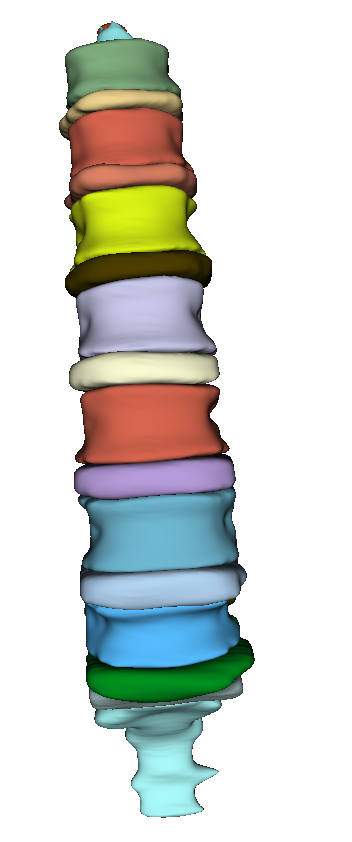
\includegraphics[height=9cm, width=\textwidth, keepaspectratio]{obrazy/case21_low_scoliosis.png}
        \caption{badanie nr 20 -- 7,95\degree{}}
        \label{fig:niewielka-skolioza-1}
    \end{subfigure}
    \hfill
    \begin{subfigure}{0.48\textwidth}
        \centering
         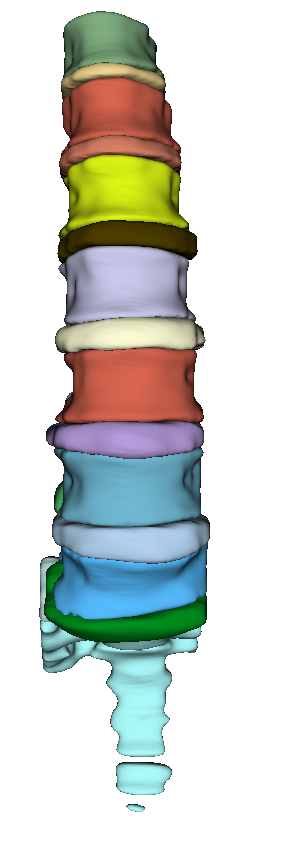
\includegraphics[height=9cm, width=\textwidth, keepaspectratio]{obrazy/case26_low_scoliosis.png}
        \caption{badanie nr 25 -- 3,72\degree{}}
        \label{fig:niewielka-skolioza-2}
    \end{subfigure}

    \vspace{0.4cm}

    \begin{subfigure}{0.48\textwidth}
        \centering
        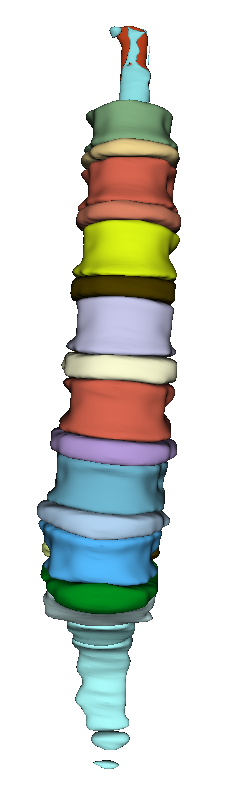
\includegraphics[height=9cm, width=\textwidth, keepaspectratio]{obrazy/case41_low_scoliosis.png}
        \caption{badanie nr 39 -- 7,91\degree{}}
        \label{fig:niewielka-skolioza-3}
    \end{subfigure}
    \hfill
    \begin{subfigure}{0.48\textwidth}
        \centering
        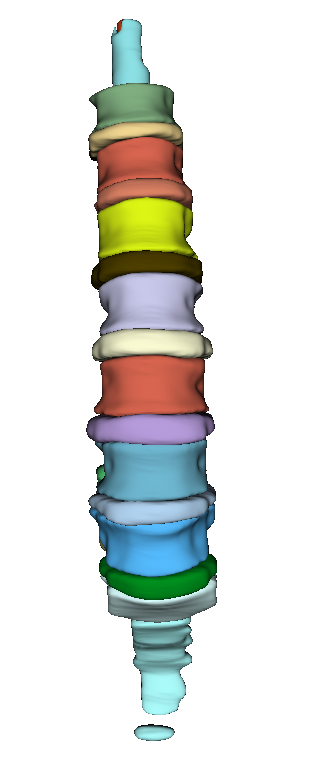
\includegraphics[height=9cm, width=\textwidth, keepaspectratio]{obrazy/case51_low_scoliosis.png}
        \caption{badanie nr 49 -- 5,58\degree{}}
        \label{fig:niewielka-skolioza-4}
    \end{subfigure}
    \captionsetup{justification=centering, font=small}
    \caption{Przykłady skrzywień opisanych jako niewielkie, dla których zmierzony kąt Cobba nie przekroczył wartości progowej}
    \label{fig:niqewielka-skolioza}
\end{figure}

Wyników fałszywie dodatnich jest siedem, a~zmierzone w~nich kąty wynoszą 8,26--17,82\degree{}.
Część z~nich nie wynika jednak z~błędu pomiaru.
W~badaniach przedstawionych na rys.~\ref{fig:prawie-skolioza} kąt Cobba przekroczył próg, a~na obrazie widoczne jest boczne wygięcie odcinka lędźwiowego, choć opis radiologiczny go nie wymienia.
Klasyfikację algorytmu można w~tych przypadkach uznać za trafne wskazanie tendencji do skoliozy, a~rozbieżność z~referencją przypisać temu, że skrzywienia niewielkiego stopnia nie zawsze trafiają do opisu badania.

\begin{figure}[H]
    \centering
    \begin{subfigure}{0.48\textwidth}
        \centering
        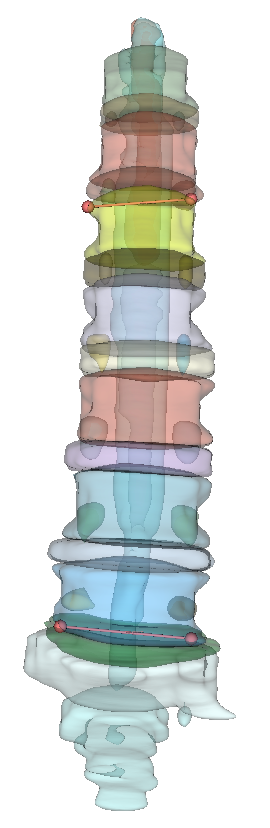
\includegraphics[height=9cm, width=\textwidth, keepaspectratio]{obrazy/case4_almost_scoliosis.png}
        \caption{badanie nr 4 -- 10,03\degree{}}
        \label{fig:prawie-skolioza-1}
    \end{subfigure}
    \hfill
    \begin{subfigure}{0.48\textwidth}
        \centering
        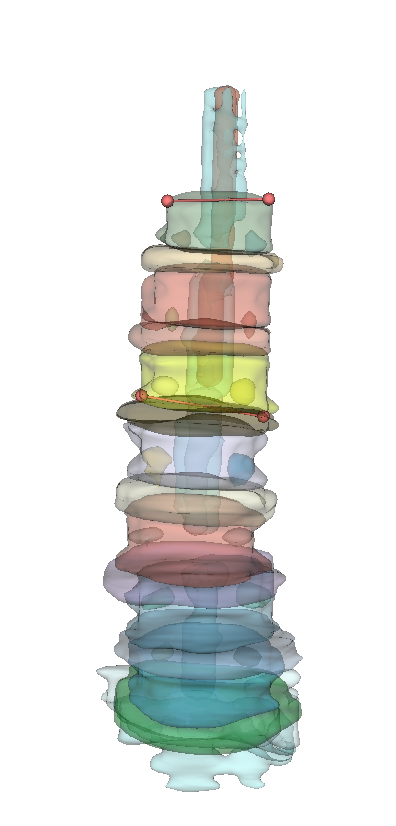
\includegraphics[height=9cm, width=\textwidth, keepaspectratio]{obrazy/case5_almost_scoliosis.png}
        \caption{badanie nr 5 -- 10,76\degree{}}
        \label{fig:prawie-skolioza-2}
    \end{subfigure}

    \vspace{0.4cm}

    \begin{subfigure}{0.48\textwidth}
        \centering
        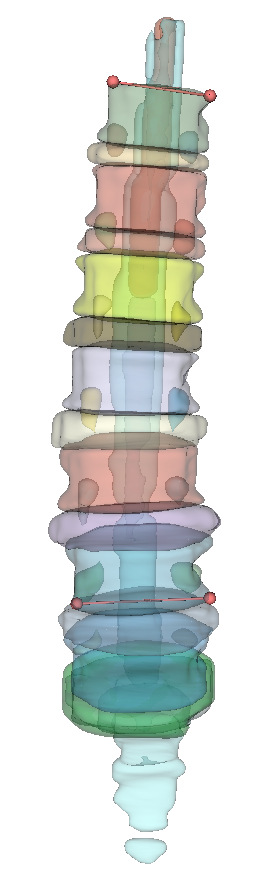
\includegraphics[height=9cm, width=\textwidth, keepaspectratio]{obrazy/case40_skolioza.png}
        \caption{badanie nr 38 -- 11,57\degree{}}
        \label{fig:prawie-skolioza-3}
    \end{subfigure}
    \hfill
    \begin{subfigure}{0.48\textwidth}
        \centering
        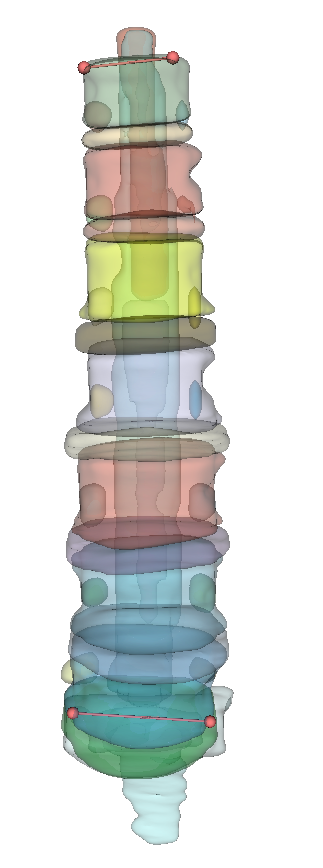
\includegraphics[height=9cm, width=\textwidth, keepaspectratio]{obrazy/case67_almost_scoliosis.png}
        \caption{badanie nr 65 -- 10,17\degree{}}
        \label{fig:prawie-skolioza-4}
    \end{subfigure}
    \captionsetup{justification=centering, font=small}
    \caption{Przykłady wyników fałszywie dodatnich -- badania bez opisanej skoliozy, w~których zmierzony kąt Cobba przekroczył wartość progową, a~obraz wskazuje na tendencję do skrzywienia bocznego}
    \label{fig:prawie-skolioza}
\end{figure}

Pomiar dla badania nr 28 odrzucono, ponieważ przy masywnej rotoskoliozie segmentacja okazała się złej jakości, a~algorytm zwrócił niewiarygodną wartość kąta 98,80\degree{} (rys.~\ref{fig:skolioza-odrzucony}).

\begin{figure}[H]
    \centering
    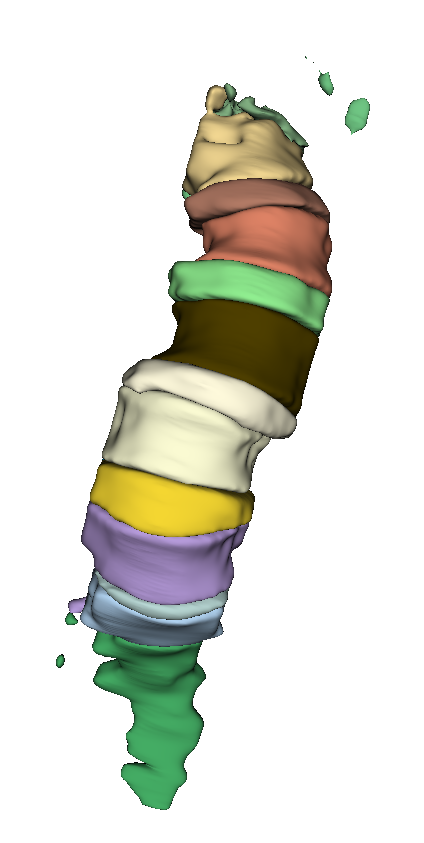
\includegraphics[height=9cm, width=0.6\textwidth, keepaspectratio]{obrazy/case28_niewiarygodny}
    \captionsetup{justification=centering, font=small}
    \caption{Badanie nr 28 -- segmentacja złej jakości przy masywnej rotoskoliozie, zmierzony kąt 98,80\degree{} (pomiar odrzucony)}
    \label{fig:skolioza-odrzucony}
\end{figure}

\subsection{Algorytm detekcji kręgozmyku i~tyłozmyku}
\label{subsec:bledy-kregozmyk}

Na rys.~\ref{fig:kregozmyk-fp} zestawiono sześć poziomów, na których algorytm wskazał ześlizg nieobecny w~opisie radiologicznym.
W~pięciu z~nich (nr 10, 35, 59, 61 i~65) przesunięcie trzonów jest widoczne na obrazie, a~w~badaniu nr 10 tyłozmyk L4/L5 potwierdził lekarz.
We wszystkich tych badaniach opisano ześlizg na innym poziomie, co sugeruje, że radiolog odnotował jedynie zmianę dominującą.
Inny charakter ma badanie nr 2, w~którym krążek L4/L5 jest wyższy w~części przedniej, przez co trzony ustawiają się nierównolegle, a~algorytm interpretuje to jako tyłozmyk.

\begin{figure}[H]
    \centering
    \begin{subfigure}{0.48\textwidth}
        \centering
        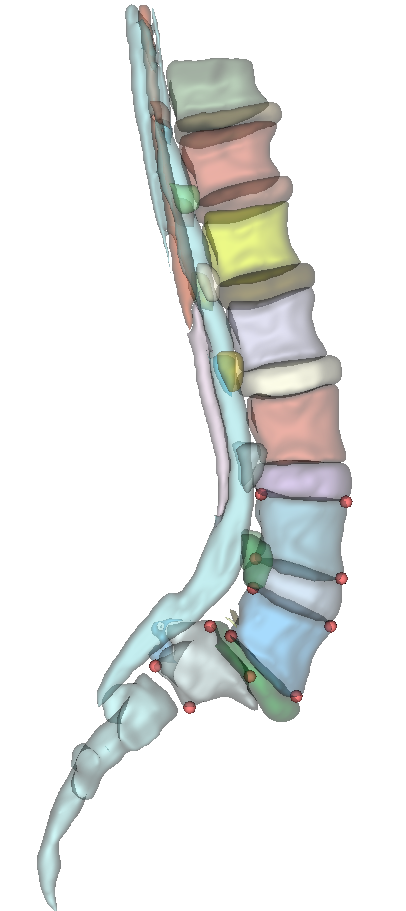
\includegraphics[height=9cm, width=\textwidth, keepaspectratio]{obrazy/zmyk/case2_tylozmyk_FP}
        \caption{badanie nr 2 -- poziom L4/L5, $s = 0,126$}
        \label{fig:kregozmyk-fp-1}
    \end{subfigure}
    \hfill
    \begin{subfigure}{0.48\textwidth}
        \centering
        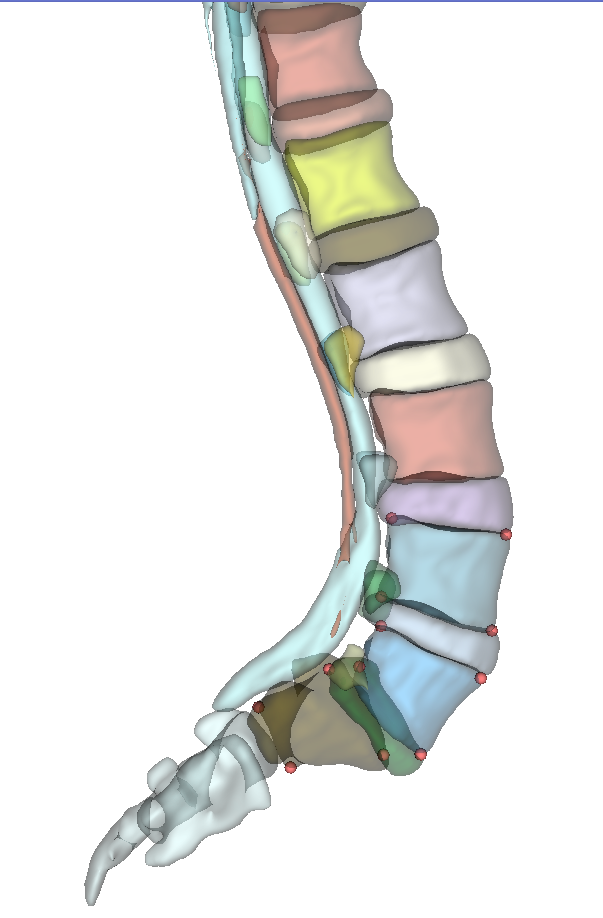
\includegraphics[height=6cm, width=\textwidth, keepaspectratio]{obrazy/zmyk/case10_FP}
        \caption{badanie nr 10 -- poziom L4/L5, $s = 0,110$}
        \label{fig:kregozmyk-fp-2}
    \end{subfigure}

    \vspace{0.4cm}

    \begin{subfigure}{0.48\textwidth}
        \centering
        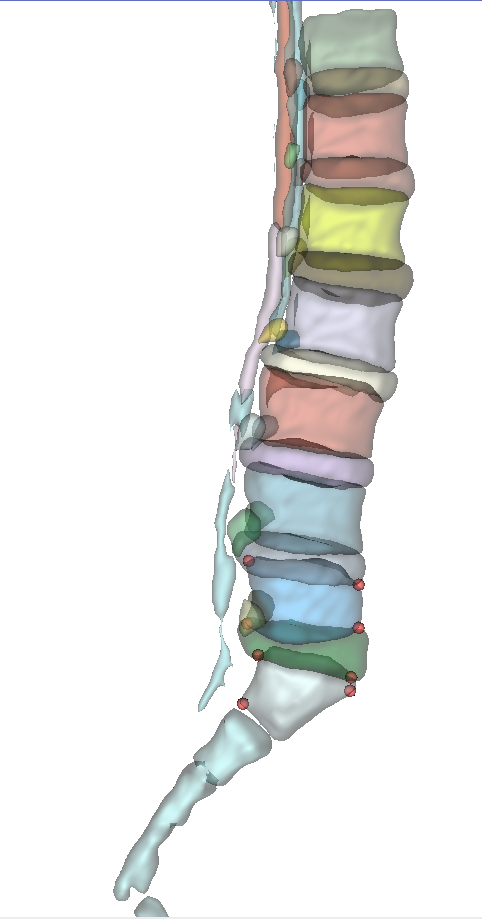
\includegraphics[height=6cm, width=\textwidth, keepaspectratio]{obrazy/zmyk/case35_FP}
        \caption{badanie nr 35 -- poziom L5/S1, $s = 0,185$}
        \label{fig:kregozmyk-fp-3}
    \end{subfigure}
    \hfill
    \begin{subfigure}{0.48\textwidth}
        \centering
        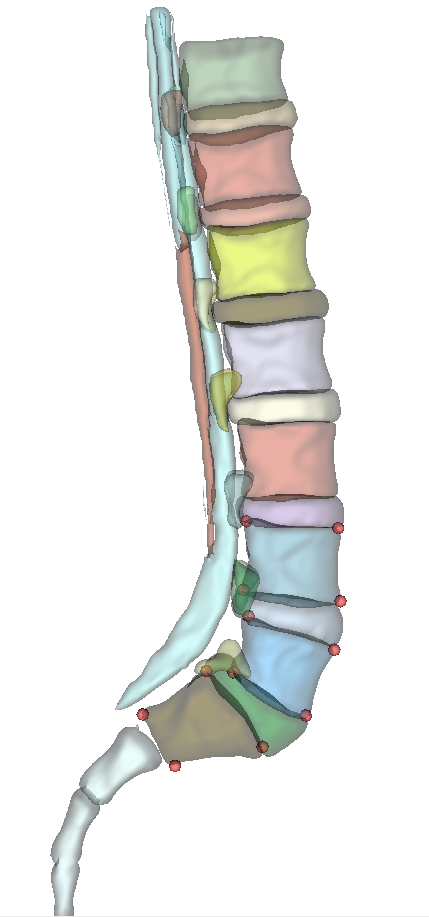
\includegraphics[height=6cm, width=\textwidth, keepaspectratio]{obrazy/zmyk/case59_FP}
        \caption{badanie nr 59 -- poziom L5/S1, $s = 0,185$}
        \label{fig:kregozmyk-fp-4}
    \end{subfigure}

    \vspace{0.4cm}

    \begin{subfigure}{0.48\textwidth}
        \centering
        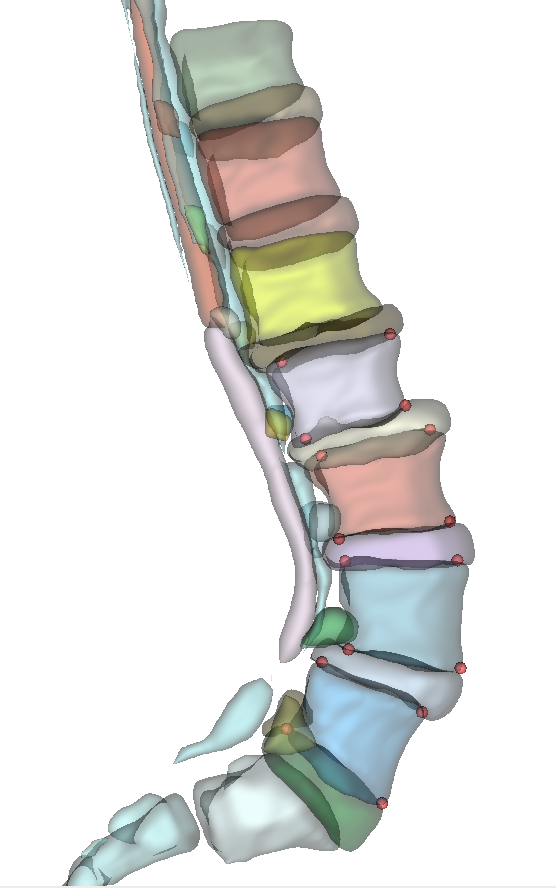
\includegraphics[height=6cm, width=\textwidth, keepaspectratio]{obrazy/zmyk/case61_FP}
        \caption{badanie nr 61 -- poziom L2/L3, $s = 0,109$}
        \label{fig:kregozmyk-fp-5}
    \end{subfigure}
    \hfill
    \begin{subfigure}{0.48\textwidth}
        \centering
        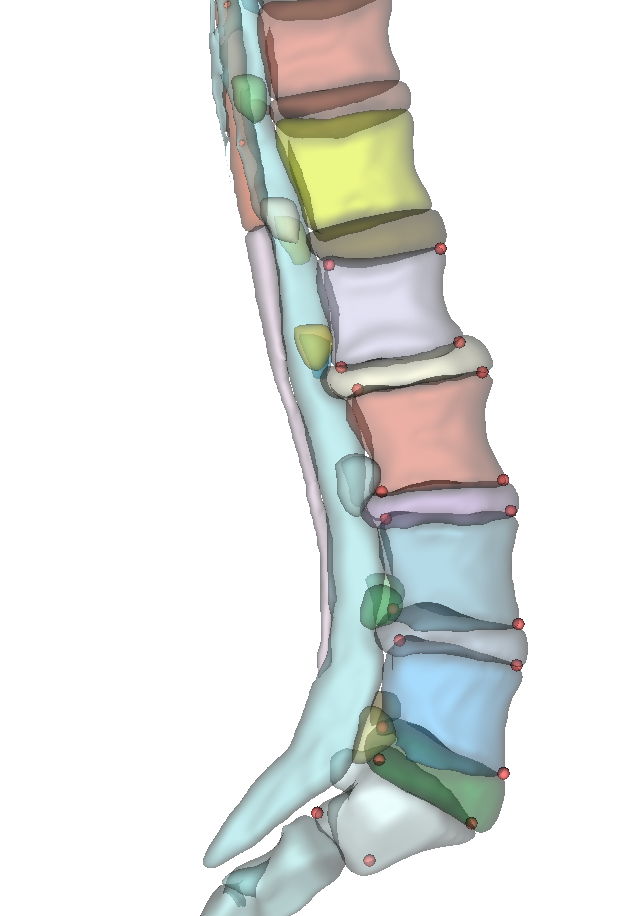
\includegraphics[height=6cm, width=\textwidth, keepaspectratio]{obrazy/zmyk/case65_FP}
        \caption{badanie nr 65 -- poziom L4/L5, $s = 0,105$}
        \label{fig:kregozmyk-fp-6}
    \end{subfigure}
    \captionsetup{justification=centering, font=small}
    \caption{Przykłady wyników fałszywie dodatnich algorytmu detekcji kręgozmyku i~tyłozmyku}
    \label{fig:kregozmyk-fp}
\end{figure}

Na rys.~\ref{fig:kregozmyk-fn} przedstawiono przykłady opisanych ześlizgów, których algorytm nie wykrył.
W~badaniu nr 3 wartość $s = 0,081$ dla tyłozmyku Th12/L1 przekracza próg kręgozmyku, ale nie wyższy próg tyłozmyku, a~w~badaniach nr 20 i~21 opisano kręgozmyk I~stopnia o~niewielkim przesunięciu, przy czym w~badaniu nr 21 trzon L5 jest zdegradowany, co utrudnia wyznaczenie jego narożników.
W~badaniu nr 8 pomiar nie był możliwy, ponieważ segmentacja nie obejmuje kości krzyżowej, a~kręgozmyk II/III stopnia występuje właśnie na poziomie L5/S1.

% Rysunek 2x2 — przypadki fałszywie ujemne (kręgozmyk/tyłozmyk).
\begin{figure}[H]
    \centering
    \begin{subfigure}{0.48\textwidth}
        \centering
        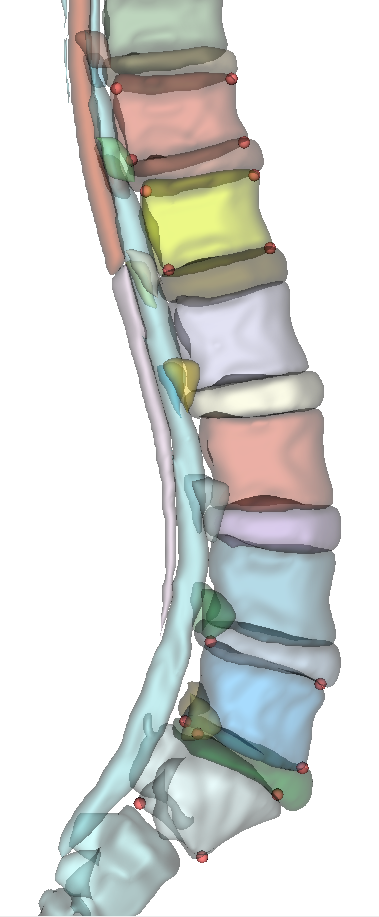
\includegraphics[height=9cm, width=\textwidth, keepaspectratio]{obrazy/zmyk/case3_th12_FN}
        \caption{badanie nr 3 -- poziom Th12/L1, $s = 0,081$}
        \label{fig:kregozmyk-fn-1}
    \end{subfigure}
    \hfill
    \begin{subfigure}{0.48\textwidth}
        \centering
        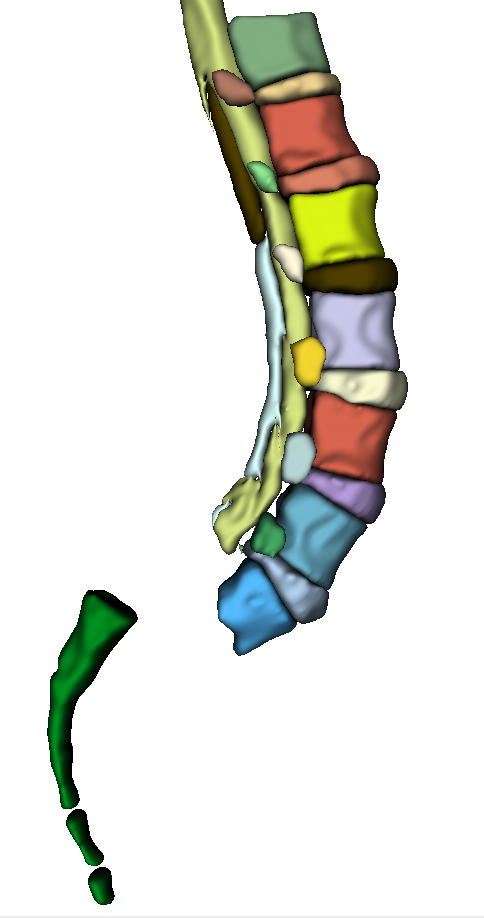
\includegraphics[height=9cm, width=\textwidth, keepaspectratio]{obrazy/zmyk/case8_nieposegmentowany_s1}
        \caption{badanie nr 8 -- poziom L5/S1, nieposegmentowany S1}
        \label{fig:kregozmyk-fn-2}
    \end{subfigure}

    \vspace{0.4cm}

    \begin{subfigure}{0.48\textwidth}
        \centering
        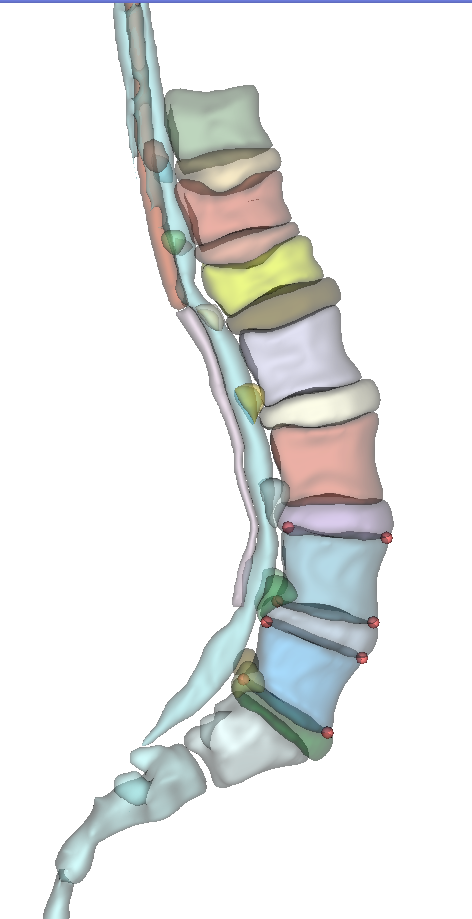
\includegraphics[height=9cm, width=\textwidth, keepaspectratio]{obrazy/zmyk/case20_FN}
        \caption{badanie nr 20 -- poziom L4/L5, $s = 0,030$}
        \label{fig:kregozmyk-fn-3}
    \end{subfigure}
    \hfill
    \begin{subfigure}{0.48\textwidth}
        \centering
        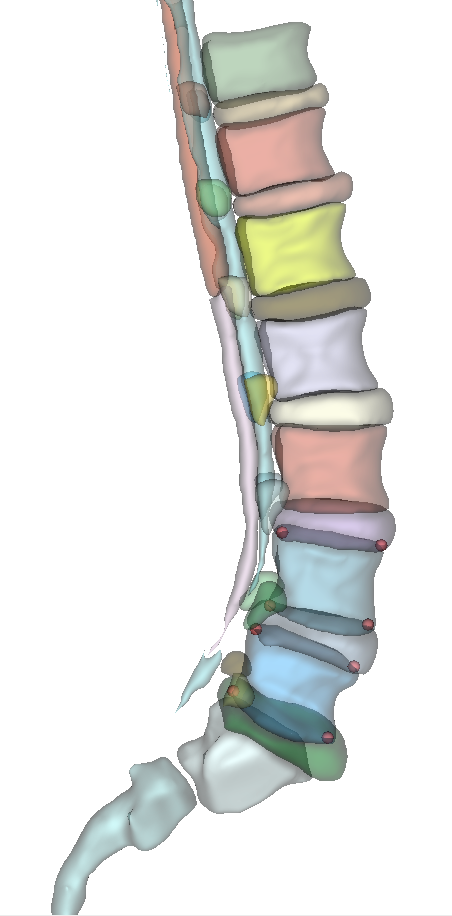
\includegraphics[height=9cm, width=\textwidth, keepaspectratio]{obrazy/zmyk/case21_FN}
        \caption{badanie nr 21 -- poziom L4/L5, $s = 0,045$}
        \label{fig:kregozmyk-fn-4}
    \end{subfigure}
    \captionsetup{justification=centering, font=small}
    \caption{Przykłady poziomów z~opisanym ześlizgiem, których algorytm nie wykrył}
    \label{fig:kregozmyk-fn}
\end{figure}

\section{Dyskusja}
\label{sec:dyskusja}

Algorytm detekcji kręgozmyku i~tyłozmyku osiągnął dokładność 0,925 przy swoistości 0,949, natomiast algorytm detekcji skoliozy -- dokładność 0,712, co wynika przede wszystkim z~płynnej granicy między normą a~niewielkim skrzywieniem.
Ocenę obu algorytmów należy jednak odczytywać z~uwzględnieniem charakteru wzorca odniesienia: opis radiologiczny jest subiektywną oceną jednego lekarza, formułowaną bez podania wartości kąta czy przesunięcia i~przy użyciu własnego, nieujawnionego progu rozpoznania.
Ocena parametrów geometrycznych kręgosłupa obarczona jest zmiennością międzyobserwatorską, wobec czego to samo badanie opisane przez innego radiologa mogłoby zostać sklasyfikowane odmiennie.
W~zebranym materiale przejawia się to zarówno w~niejednoznacznych określeniach \enquote{niewielka} czy \enquote{dyskretna} skolioza, stosowanych przy bardzo różnych kątach, jak i~w~ześlizgach widocznych na obrazie i~wskazanych przez algorytm, lecz pominiętych w~opisie.
Drugim czynnikiem ograniczającym jest jakość segmentacji, ponieważ algorytmy operują na mapie etykiet, a~nie na samym obrazie -- brak kości krzyżowej (badanie nr 8), zniekształcony trzon (nr 21) czy błędna segmentacja przy masywnej rotoskoliozie (nr 28) przenoszą się bezpośrednio na wynik.
Największą trudność sprawiają przypadki graniczne -- skrzywienia o~kącie bliskim progu oraz przesunięcia o~wartości $s$ między 0,06 a~0,10 -- które także lekarz weryfikujący wyniki oceniał jako niejednoznaczne.
Mimo tych ograniczeń oba algorytmy stanowią wartościowe narzędzie wspomagające: analiza pojedynczego badania trwa około 1,7~s, wynik ma postać powtarzalnej wartości liczbowej.
